\documentclass{article}
\usepackage{xcolor}
\usepackage{titleps}
\usepackage[letterpaper, margin=0.95in]{geometry}
\usepackage{url}
\usepackage{amsmath}
\usepackage{amssymb}
\usepackage{wrapfig}
\usepackage{float}
\usepackage{mathtools}
\usepackage{enumitem}
\usepackage{tabu}
\usepackage{parskip}
\usepackage{natbib}
\usepackage{listings}
\usepackage[utf8]{inputenc} % allow utf-8 input
\usepackage[T1]{fontenc}    % use 8-bit T1 fonts
\usepackage[hidelinks]{hyperref}       % hyperlinks
\usepackage{wrapfig}
\usepackage{url}            % simple URL typesetting
\usepackage{booktabs}       % professional-quality tables
\usepackage{amsfonts}       % blackboard math symbols
\usepackage{nicefrac}       % compact symbols for 1/2, etc.
\usepackage{microtype}      % microtypography
\usepackage{xcolor}         % colors
\usepackage{amsmath,amssymb} % define this before the line numbering.
\usepackage{makecell}
% % Support for easy cross-referencing
\usepackage{graphics} % for pdf, bitmapped graphics files
\usepackage{colortbl}
\usepackage{xcolor}
% \usepackage{epsfig} % for postscript graphics files
\usepackage{empheq}
%\usepackage{mathptmx} % assumes new font selection scheme installed
% \usepackage{times} % assumes new font selection scheme installed
\usepackage{bm}
\usepackage{bbding} 
% \usepackage{cite}
\usepackage{diagbox}
\usepackage[linesnumbered,ruled]{algorithm2e}
% \usepackage{ulem} %to strike the words
% \usepackage{hyperref}
% \usepackage{soul}

\newcommand{\cmark}{\ding{51}}%
\newcommand{\xmark}{\ding{55}}%
% \definecolor{themeblue}{RGB}{57, 162, 219}
% \definecolor{themegreen}{RGB}{87, 204, 153}
% \definecolor{forestgreen}{RGB}{47, 159, 87}

\usepackage[capitalize]{cleveref}
% \usepackage{todonotes}
\usepackage{float}
\usepackage{booktabs}
\usepackage{multirow}
%\usepackage{ bbold }
\usepackage{mathrsfs}
\usepackage[utf8]{inputenc}
%\usepackage{subfigure}
\usepackage{pifont}
\usepackage{threeparttable}

\usepackage{hyperref}
\usepackage[color=red]{todonotes}
\usepackage{forest}
\definecolor{light-yellow}{HTML}{FFE5CC}
\newcounter{RNum}
\renewcommand{\theRNum}{\arabic{RNum}}
\newcommand{\Remark}{\noindent\textbf{Remark}~\refstepcounter{RNum}\textbf{\theRNum}: }
\newcommand{\fref}[1]{Fig.~\ref{#1}}
\newcommand{\sref}[1]{Section~\ref{#1}}
\newcommand{\tref}[1]{Table~\ref{#1}}
\newcommand{\appref}[1]{Appendix~\ref{#1}}
\newcommand{\highlight}[1]{\noindent\quad\textbf{#1}:~}
\newcommand{\myparagraph}[1]{\noindent\textbf{#1}~}

\newpagestyle{ruled}
{\sethead{CMU 16-831}{Intro to Robot Learning}{Fall 2024}\headrule
  \setfoot{}{}{}}
\pagestyle{ruled}

\renewcommand\makeheadrule{\color{black}\rule[-.75\baselineskip]{\linewidth}{0.4pt}}
\renewcommand*\footnoterule{}

\begin{document}
\lstset{basicstyle = \ttfamily,columns=fullflexible,
backgroundcolor = \color{light-yellow}
}

\begin{centering}
    {\Large Assignment 1: Imitation Learning} \\
    \vspace{.25cm}
    \textbf{Andrew ID:} \texttt{yulongl} \\
    \textbf{Collaborators:} \texttt{N/A}\\ 
\end{centering}

\vspace{.5cm}

\section{Behavioral Cloning (65 pt)}
\subsection{Part 2 (10 pt)}
\begin{table}[!h]
  \centering
  \caption{Report your result in this table.}
    \begin{tabular}{cccccc}
    \toprule[1.0pt]
    Metric/Env & Ant-v2 & Humanoid-v2 & Walker2d-v2 & Hopper-v2 & HalfCheetah-v2 \\
    \midrule
    Mean  & 4713.653 & 10344.518 & 5566.846 & 3772.670 & 4205.778 \\
    Std.  & 12.197 & 20.981 & 9.238 & 1.948 & 83.039 \\
    \bottomrule[1.0pt]
    \end{tabular}%
  \label{tab:p2}%
\end{table}%

\subsection{Part 3 (35 pt)}
\begin{table}[htbp]
  \centering
  \caption{Fill your results in this table.}
    \begin{tabular}{ccccc}
    \toprule[1.0pt]
    Env   & \multicolumn{2}{c}{Ant-v2} & \multicolumn{2}{c}{Humanoid-v2} \\
    \midrule
    Metric & Mean  & Std.  & Mean  & Std. \\
    Expert & 4713.653 & 12.197 & 10344.518 & 20.981 \\
    BC    & 1729.545 & 767.105 &  281.326 & 15.861 \\
    \bottomrule[1.0pt]
    \end{tabular}%
  \label{tab:p3}%
  \caption{BC agent performance with 3 layers MLP of width 256, trained for 1000 steps.}
\end{table}%

\subsection{Part 4 (20 pt)}

The graph shows how the BC agent's performance varies with the MLP width. We can see that the performance increases as the width increases initially, which makes sense because a wider network has more parameters to learn from the data. However, after a certain point, the performance starts to decrease. This is because the network becomes too large and starts to overfit to the data.


\begin{figure*}[!h]
	\centering
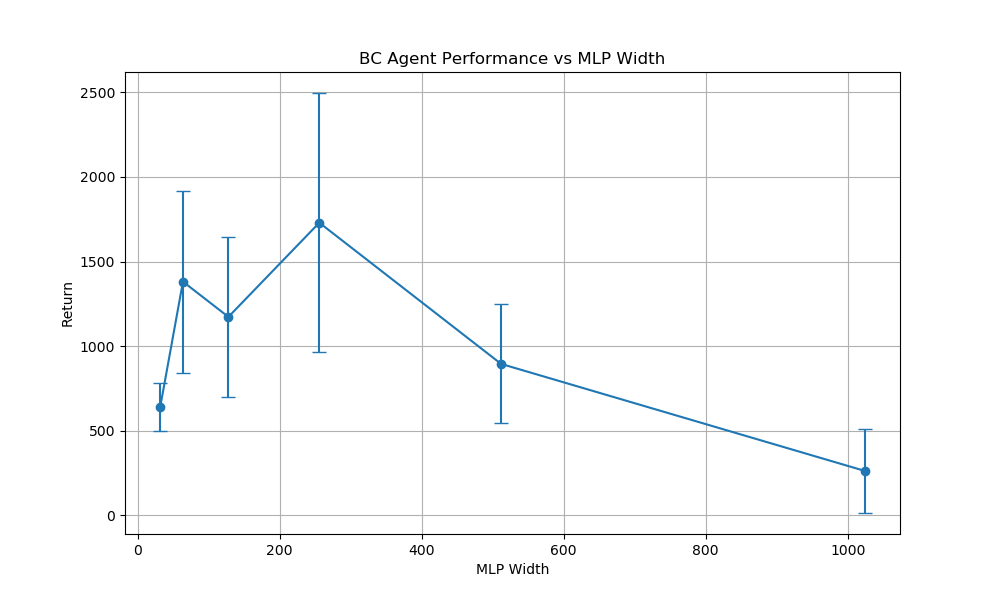
\includegraphics[width=0.5\columnwidth]{../hw1/rob831/scripts/bc_agent_performance_vs_mlp_width.png}
	\caption{BC agent’s performance varies with the value of MLP width in Ant-v2 environment.}
	\label{fig:p4}
\end{figure*}

\section{DAgger (35 pt)}
\subsection{Part 2 (35 pt)}

\begin{figure*}[!h]
	\centering
	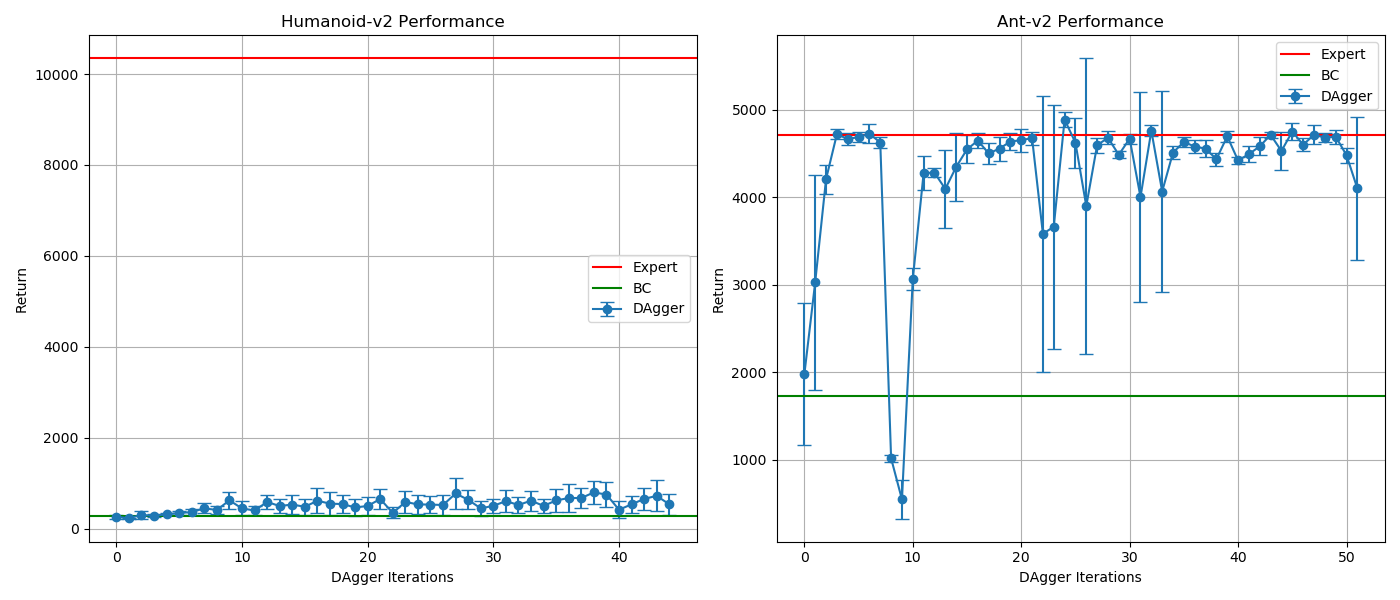
\includegraphics[width=1.0\columnwidth]{../hw1/rob831/scripts/dagger_performance.png}
	\caption{BC with DAgger performance with 2 layers MLP of width 64, trained for 1000 steps per iterations.}
	\label{fig:p5}
\end{figure*}

\end{document}